\documentclass{standalone}
\usepackage{graphicx}	
\usepackage{amssymb, amsmath}
\usepackage{color}

\usepackage{tikz}
\usetikzlibrary{intersections, backgrounds, math}
\usepackage{pgfmath}

\definecolor{light}{RGB}{220, 188, 188}
\definecolor{mid}{RGB}{185, 124, 124}
\definecolor{dark}{RGB}{143, 39, 39}
\definecolor{highlight}{RGB}{180, 31, 180}
\definecolor{light_teal}{RGB}{107, 142, 142}
\definecolor{mid_teal}{RGB}{72, 117, 117}
\definecolor{dark_teal}{RGB}{29, 79, 79}
\definecolor{gray10}{gray}{0.1}
\definecolor{gray20}{gray}{0.2}
\definecolor{gray30}{gray}{0.3}
\definecolor{gray40}{gray}{0.4}
\definecolor{gray60}{gray}{0.6}
\definecolor{gray70}{gray}{0.7}
\definecolor{gray80}{gray}{0.8}
\definecolor{gray90}{gray}{0.9}
\definecolor{gray95}{gray}{0.95}

\begin{document}

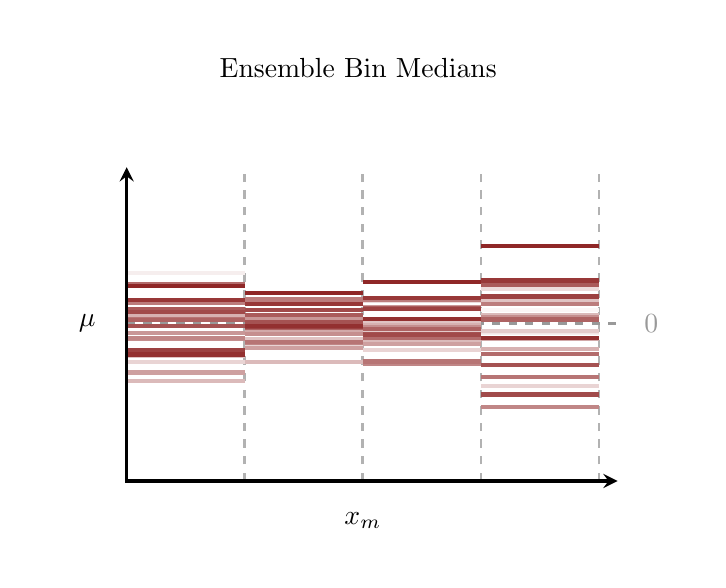
\begin{tikzpicture}[scale=1.0]

  \begin{scope}[shift={(0, -6.75)}]
    \draw[white] (-4.25, -3) rectangle (4.25, 3.75);
    
    \node[align=center] at (0, 3.25) { Ensemble Bin Medians };
    
    \foreach \b in {-3.0, -1.5,  0.0,  1.5,  3.0} {
      \draw[gray70, dashed, line width=1] (\b, -2) -- (\b, 2);
    }
    
    \draw[gray60, dashed, line width=1] (-3, 0) -- (3.25, 0);   
    \node[gray60, anchor=west] at (3.1, 0)  { $\quad 0$ };
    
    \foreach \a/\b/\c/\d [count=\n] in {-0.368/0.003/0.192/0.170, 0.639/0.266/0.010/-0.120,
                                        0.078/-0.096/-0.157/-0.101, 0.090/0.170/0.281/0.436,
                                        -0.486/-0.263/-0.341/-0.789, 0.176/-0.026/-0.122/-0.095,
                                        -0.410/-0.194/0.033/0.288, -0.726/-0.490/-0.221/0.105,
                                        0.092/0.106/-0.019/-0.321, -0.336/-0.111/-0.059/-0.196,
                                        -0.623/-0.314/-0.264/-0.524, -0.116/0.059/0.209/0.340,
                                        -0.195/-0.136/-0.048/0.082, -0.182/-0.243/-0.516/-1.065,
                                        0.265/0.304/0.301/0.245, 0.057/-0.238/-0.483/-0.681,
                                        0.501/0.109/-0.187/-0.382, 0.042/-0.061/-0.065/0.050,
                                        0.180/0.110/0.193/0.490, -0.030/0.014/-0.135/-0.528,
                                        0.146/0.171/-0.147/-0.901, -0.339/-0.048/0.179/0.343, 
                                        0.303/0.252/0.319/0.547, -0.393/-0.029/0.052/-0.183,
                                        0.473/0.388/0.530/0.979} {
       \pgfmathsetmacro{\prop}{4 * \n};
       \colorlet{custom}{dark!\prop!white};
       \draw[custom, line width=1.5] (-3, \a)   -- (-1.5, \a);
       \draw[custom, line width=1.5] (-1.5, \b) -- (0, \b);
       \draw[custom, line width=1.5] (0, \c)    -- (1.5, \c);
       \draw[custom, line width=1.5] (1.5, \d)  -- (3, \d);
    }
     
    \draw [->, >=stealth, line width=1.25] (-3.00, -2.015) -- +(0, 4);
    \draw [->, >=stealth, line width=1.25] (-3.015, -2.00) -- +(6.25, 0);
    
    \node at (-3.5, 0) { $\mu$ };
    \node at (0, -2.5) { $x_{m}$ };
  \end{scope}
  
\end{tikzpicture}

\end{document}  